\section{Durchführung}
\label{sec:Durchführung}
Für die experimentellen Bestimmung der Suszeptibilität verschiedener Stoffe wird eine Schaltung verwendet, die in \autoref{fig:Schaltung2} zu sehen ist.
Um Störspannungen zu vermindern und das Signal der Brückenschaltung zu verstärken, wird ein Selektivverstärker verwendet. Da dieser Filter nur einen 
bestimmmten Frequenzbereich an Wechselspannungen durchlässt, muss die Frequenz des Sinusgenerators genau auf den Selektivverstärker abgestimmt werden.

\begin{figure}
    \centering
    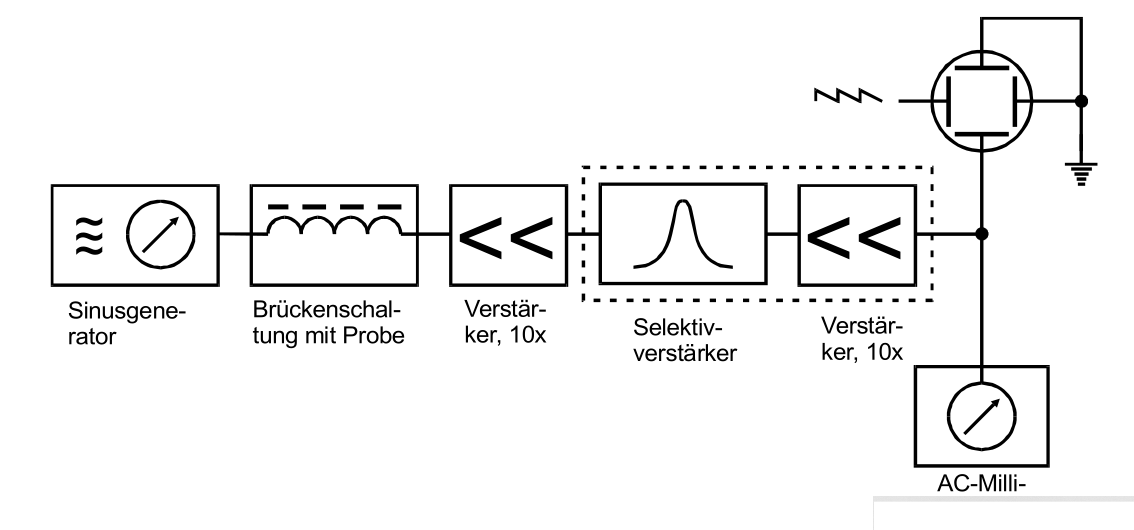
\includegraphics[width = .8\textwidth]{content/Schaltung2.png}
    \caption{Blockschaltplan des Versuchaufbaus. \cite{v606}}
    \label{fig:Schaltung2}
\end{figure}

\subsection{Untersuchung der Filterkurve des Selektivverstärkers}
\label{subsec:D_Filterkurve}
Zur Bestimmung der Filterkurve wird ein Sinusgenerator an den Selektivverstärker angeschlossen, mit welchem Frequenzen im Bereich von $15$ bis $\qty{40}{\kilo\hertz}$
erzeugt werden können. Der Ausgang des Verstärkers wird mit einem Spannungsmessgerät (Voltmeter) verbunden. Gemessen wird im einstelligen Voltbereich.
Zuerst kann die Lage des Spannungsmaximums grob ermittelt werden. Hierzu kann bei Bedarf ein Oszilloskop anstelle des Voltmeters verwendet werden.
Um die Filterkurve auszumessen, wird ein ausreichend großer Frequenzbereich um die Frequenz des Spannungsmaximums gewählt. Es werden Messwertepaare der Frequenz
und der gemessenen Spannung notiert, wobei in der näheren Umgebung des Maximums mehr Messwerte bestimmmt werden sollten, da in diesem Bereich eine starke Steigung 
des Graphen zu erwarten ist.
Aus den Messwerten lässt sich die Filterkurve des Selektivverstärkers ermitteln, indem die Spannung als Funktion der Frequenz aufgetragen wird.

\subsection{Messreihe zur Bestimmung der Suszeptibilität}
\label{subsec:D_Suszeptibilität}
Wie in \autoref{sec:Theorie} beschrieben kann die Suszeptibilität paramagnetischer Stoffe auf zwei verschiedene Weisen experimentell bestimmmt werden. 
Die benötigten Messwerte zu den beiden Verfahren können derselben Messreihe entnommen werden. 

Da die verwendeten Proben in Pulverform vorliegen und so nicht die Dichte eines Einkristalles selbigen Materials erreichen, muss zunächst diese Abweichung
rechnerisch kompensiert werden. Dazu wird der Querschnitt $Q_\text{real}$ der Probe bestimmt, den sie als Einkristall mit entsprechender Dichte hätte,
indem der gemessene Querschnitt mit dem Verhältnis $\sfrac{\rho_\text{P}}{\rho_\text{E}}$ der Dichten der Probe $\rho_\text{P}$ und des Einkristalles $\rho_\text{E}$ 
multipliziert wird. Da $\rho = \sfrac{M}{V}$ ($M$: Masse, $V$: Volumen) gilt, kann der effektive Querschnitt über
\begin{equation}
    \label{eqn:Q_real}
    Q_\text{real} = \frac{M_\text{P}}{l \rho_\text{E}}
\end{equation}
berechnet werden.

Aus diesem Grund wird die Länge $l$ jeder Probe zuvor bestimmt. 

Die aus der Filterkurve bestimmte Frequenz des Spannungsmaximums wird an dem Sinusgenerator eingestellt. Da ein anderer Spannungsgenerator verwendet wird, sollte 
überprüft werden, ob tatsächlich das Maximum der Spannung vorliegt.

Vor jeder Messung wird mithilfe des regelbaren Widerstands $R_\text{P}$ die gemessene Spannung auf ein Minimum geregelt. Der eingestellte Widerstand und die angezeigte 
Spannung werden notiert. Anschließend wird das Proberöhrchen in die dafür vorgesehene Öffnung eingeführt und die nun gemessene Spannung vermerkt. 
Dieser Wert bietet eine der zwei Möglichkeiten zur experimentellen Bestimmung der Suszeptibilität. Über den Widerstand $R_\text{P}$ kann wieder ein Minimum der Spannung
eingestellt werden. Aus diesem Wert kann ebenfalls die Suszeptibilität des Stoffes bestimmmt werden. Auch die zugehörige Spannung wird wieder notiert.
Dieses Vorgehen wird für jede Probe drei Mal durchgeführt. Insgesamt werden Proben drei verschiedener Stoffe untersucht.  
